%%%
%%%%%%%%%%%%%%%%%%%%%%%%%%%%%%%%%%%%%%%%%%%%%%%%%%%%%
%%% Draft paper for Diversity, Equity, and Inclusion in HRI
%%% https://sites.google.com/view/dei-hri/call-for-papers
%%% Important dates 
%%% Deadline January 30th, 2023 (final extension)
%%% Paper Acceptance Notification: February 13th, 2023 (final extension)
%%% Camera-Ready Paper: March 1st, 2023
%%%
%%%
%%%%%%%%%%%%%%%%%%%%%%%%%%%%%%%%%%%%%%%%%%%%%%%%%%%%%
%%% Roadmap for dei-hri2023:
%%% 1. Setting template and draft sections: 14-to-15-Jan-2023
%%% 2. Distillation: 15-to-20-Jan
%%% 3. 25min-ish google-meeeting: 19-Jan 15:00/Mex; 21:00/UK; 13:00/Vancouver; 22:00/Spain; 13:00/PST 
%%% 4. Send second draft Friday 20th Jan
%%% 5. Submission: 23th Jan 2023: 
%%%
%%%
%%%
%%%%%%%%%%%%%%%%%%%%%%%%%%%%%%%%%%%%%%%%%%%%%%%%%%%%%
%%% Overleaf project
%%% Anyone with this link can edit this project
%%% https://www.overleaf.com/3395627816xdvrymdbqqft
%%%
%%%%%%%%%%%%%%%%%%%%%%%%%%%%%%%%%%%%%%%%%%%%%%%%%%%%%
%%% Instrucitons for overleaf project
%%% Overleaf might be new to you, but it is quite easy to use. 
%%% 1. Go to the section where you want to write up in the PDF paper and double click that will point you to the text editor. 
%%% 2. Make edition as in word, and
%%% 3. Prese Ctrl+s to save and compile your changes in the PDF document.
%%% 4. After Ctrl+s, all should be saved and ready for others to see, to review, etc.
%%% Ps. Using percentage symbol is consdiered as comment and it is not apearing in the PDF version of the paper.
%% Don't worry about adding new references `\cite{}`, we can add them later.
%%% Thanks, Miguel
%%%
%%%
%%%%%%%%%%%%%%%%%%%%%%%%%%%%%%%%%%%%%%%%%%%%%%%%%%%%%
%%% Github project:
%%% https://github.com/air4children/dei-hri2023/  
%%%
%%%
%%%
%%%
%%%

%%%%%%%%%%%%%%%%%%%%%%%%%%%%%%%%%%%%%%%%%%%%%%%%%%%%%
%% This is file `main.tex',
%% generated with the docstrip utility.
%%
%% The original source files were:
%%
%% samples.dtx  (with options: `manuscript')
%% 
%% IMPORTANT NOTICE:
%% 
%% For the copyright see the source file.
%% 
%% Any modified versions of this file must be renamed
%% with new filenames distinct from sample-manuscript.tex.
%% 
%% For distribution of the original source see the terms
%% for copying and modification in the file samples.dtx.
%% 
%% This generated file may be distributed as long as the
%% original source files, as listed above, are part of the
%% same distribution. (The sources need not necessarily be
%% in the same archive or directory.)
%%
%% Commands for TeXCount
%TC:macro \cite [option:text,text]
%TC:macro \citep [option:text,text]
%TC:macro \citet [option:text,text]
%TC:envir table 0 1
%TC:envir table* 0 1
%TC:envir tabular [ignore] word
%TC:envir displaymath 0 word
%TC:envir math 0 word
%TC:envir comment 0 0
%%
%%
%% The first command in your LaTeX source must be the \documentclass command.
%%%% Small single column format, used for CIE, CSUR, DTRAP, JACM, JDIQ, JEA, JERIC, JETC, PACMCGIT, TAAS, TACCESS, TACO, TALG, TALLIP (formerly TALIP), TCPS, TDSCI, TEAC, TECS, TELO, THRI, TIIS, TIOT, TISSEC, TIST, TKDD, TMIS, TOCE, TOCHI, TOCL, TOCS, TOCT, TODAES, TODS, TOIS, TOIT, TOMACS, TOMM (formerly TOMCCAP), TOMPECS, TOMS, TOPC, TOPLAS, TOPS, TOS, TOSEM, TOSN, TQC, TRETS, TSAS, TSC, TSLP, TWEB.
% \documentclass[acmsmall]{acmart}

%%%% Large single column format, used for IMWUT, JOCCH, PACMPL, POMACS, TAP, PACMHCI
% \documentclass[acmlarge,screen]{acmart}

%%%% Large double column format, used for TOG
% \documentclass[acmtog, authorversion]{acmart}

%%%% Generic manuscript mode, required for submission
%%%% and peer review

%\documentclass[manuscript,screen,review]{acmart}
%\documentclass[sigconf,authordraft]{acmart}
%\documentclass[sigconf,review]{acmart}
% \documentclass[sigconf,anonymous,review]{acmart}
\documentclass[sigconf]{acmart}
%\documentclass[sigconf,review]{acmart}
%\documentclass[sigchi-a,anonymous,review]{acmart}
%\documentclass[acmconf,anonymous,review]{acmart}

%sigchi: Used for SIGCHI conference articles.
%sigchi-a: Used for SIGCHI “Extended Abstract” articles.
%sigplan: Used for SIGPLAN conference articles.


\graphicspath{{../figures}} %goes to path: figures/

%% Fonts used in the template cannot be substituted; margin 
%% adjustments are not allowed.
%%
%% \BibTeX command to typeset BibTeX logo in the docs
\AtBeginDocument{%
  \providecommand\BibTeX{{%
    \normalfont B\kern-0.5em{\scshape i\kern-0.25em b}\kern-0.8em\TeX}}}

%% Rights management information.  This information is sent to you
%% when you complete the rights form.  These commands have SAMPLE
%% values in them; it is your responsibility as an author to replace
%% the commands and values with those provided to you when you
%% complete the rights form.
\setcopyright{acmcopyright}
\copyrightyear{2023}
\acmYear{2023}
\acmDOI{XXXXXXX.XXXXXXX}

%% These commands are for a PROCEEDINGS abstract or paper.
\acmConference[HRI '23]{Make sure to enter the correct
  conference title from your rights confirmation emai}{March 13--16,
  2023}{Stockholm, SE}
%
%  Uncomment \acmBooktitle if th title of the proceedings is different
%  from ``Proceedings of ...''!
%
\acmBooktitle{HRI '23: ACM/IEEE International Conference on Human-Robot Interaction, 
March 13-16, 2023 Stockholm, SE} 
\acmPrice{15.00}
\acmISBN{978-1-4503-XXXX-X/18/06}


%%
%% Submission ID.
%% Use this when submitting an article to a sponsored event. You'll
%% receive a unique submission ID from the organizers
%% of the event, and this ID should be used as the parameter to this command.
%%\acmSubmissionID{123-A56-BU3}

%%
%% For managing citations, it is recommended to use bibliography
%% files in BibTeX format.
%%
%% You can then either use BibTeX with the ACM-Reference-Format style,
%% or BibLaTeX with the acmnumeric or acmauthoryear sytles, that include
%% support for advanced citation of software artefact from the
%% biblatex-software package, also separately available on CTAN.
%%
%% Look at the sample-*-biblatex.tex files for templates showcasing
%% the biblatex styles.
%%

%%
%% The majority of ACM publications use numbered citations and
%% references.  The command \citestyle{authoryear} switches to the
%% "author year" style.
%%
%% If you are preparing content for an event
%% sponsored by ACM SIGGRAPH, you must use the "author year" style of
%% citations and references.
%% Uncommenting
%% the next command will enable that style.
%%\citestyle{acmauthoryear}

%%
%% end of the preamble, start of the body of the document source.
\begin{document}

%%
%% The "title" command has an optional parameter,
%% allowing the author to define a "short title" to be used in page headers.
\title{
%How to teach bias in AI and Robotics to Mexican Children?%Sun 15 Jan 07:22:56 GMT 2023
% Teaching bias in AI and Robotics to Mexican Children%Sun 15 Jan 08:25:41 GMT 2023
%Teaching bias in AI and Robotics to Children in a small community in Mexico
%Fri 20 Jan 06:15:26 GMT 2023
Teaching AI and Robotics to Children in a Mexican town
%Mon 23 Jan 23:57:27 GMT 2023
}

%%
%% The "author" command and its associated commands are used to define
%% the authors and their affiliations.
%% Of note is the shared affiliation of the first two authors, and the
%% "authornote" and "authornotemark" commands
%% used to denote shared contribution to the research.
\author{Antonio Badillo-Perez}
\affiliation{%
  \institution{air4children}
  \city{Xicohtzinco, Tlaxcala}
  \country{M\'exico}}

\author{Donato Badillo-Perez}
\affiliation{%
  \institution{air4children}
  \city{Xicohtzinco, Tlaxcala}
  \country{M\'exico}}
  
% \author{Antonio Badillo-Perez}
% \authornote{Both authors contributed equally to this research.}
% \email{trovato@corporation.com}
% \orcid{1234-5678-9012}
% \author{G.K.M. Tobin}
% \authornotemark[1]
% \email{webmaster@marysville-ohio.com}
% \affiliation{%
%   \institution{Institute for Clarity in Documentation}
%   \streetaddress{P.O. Box 1212}
%   \city{Dublin}
%   \state{Ohio}
%   \country{USA}
%   \postcode{43017-6221}
% }


\author{Alex Barco}
\affiliation{%
  \institution{University of Deusto} %Engineering Faculty, 
  % \streetaddress{1 Th{\o}rv{\"a}ld Circle}
  \city{Bilbao Biscay}
  \country{Spain}}
% \email{jsmith@affiliation.org}

\author{Rocio Montenegro}
\affiliation{%
  \institution{Family Montessori School Society}
  % \streetaddress{8600 Datapoint Drive}
  \city{Vancouver, British Columbia} 
  % \state{Texas}
  \country{Canada}
  % \postcode{78229}
  }
% \email{cpalmer@prl.com}

\author{Miguel Xochicale}
\affiliation{%
  \institution{air4children}
  \city{Xicohtzinco, Tlaxcala}
  \country{M\'exico}}
\email{air4children@gmail.com}

%%
%% By default, the full list of authors will be used in the page
%% headers. Often, this list is too long, and will overlap
%% other information printed in the page headers. This command allows
%% the author to define a more concise list
%% of authors' names for this purpose.
\renewcommand{\shortauthors}{Xochicale M. et al.}

%%
%% The abstract is a short summary of the work to be presented in the
%% article.
\begin{abstract}
In this paper, we present a pilot study aiming to investigate the challenges of teaching AI and Robotics to children in  low- and middle-income countries.
Challenges such as the little to none experts and the limited resources in a Mexican town to teach AI and Robotics were addressed with
the creation of inclusive learning activities with Montessori method and open-source educational robots.
 % teaching bias in AI and
For the pilot study, we invited 14 participants of which 10 were able to attend, 6 male and 4 female of (age in years: mean=8 and std=$\pm$1.61) and four instructors of different teaching experience levels to young audiences.
We reported results of a four-lesson curriculum that is both inclusive and engaging. 
% with Montessori method and low-cost open source educational robots. 
We showed the impact on the increase of general agreement of participants on the understanding of what engineers and scientists do in their jobs, with engineering attitudes surveys and Likert scale charts from the first and the last lesson.
We concluded that this pilot study helped children coming from low- to mid-income families to learn fundamental concepts of AI and Robotics and aware them of the potential of AI and Robotics applications which might rule their adult lives.
Future work might lead (a) to have better understanding on the financial and logistical challenges to organise a workshop with a major number of participants for reliable and representative data and (b) to improve pretest-posttest survey design and its statistical analysis.
The resources to reproduce this work are available at \url{https://github.com/air4children/dei-hri2023}.
\end{abstract}
%of teaching AI and Robotics in a community where little to none experts were able to taught such subjects, and the challenges of creating a curriculum 


%%
%% The code below is generated by the tool at http://dl.acm.org/ccs.cfm.
%% Please copy and paste the code instead of the example below.
%%
\begin{CCSXML}
<ccs2012>
     <concept>
         <concept_id>10003120.10003121.10011748</concept_id>
         <concept_desc>Human-centered computing~Empirical studies in HCI</concept_desc>
         <concept_significance>500</concept_significance>
         </concept>
     <concept>
         <concept_id>10003120.10011738.10011776</concept_id>
         <concept_desc>Human-centered computing~Accessibility systems and tools</concept_desc>
         <concept_significance>500</concept_significance>
         </concept>
     <concept>
         <concept_id>10010405.10010489.10010491</concept_id>
         <concept_desc>Applied computing~Interactive learning environments</concept_desc>
         <concept_significance>300</concept_significance>
         </concept>
     <concept>
         <concept_id>10003456.10010927.10010930.10010931</concept_id>
         <concept_desc>Social and professional topics~Children</concept_desc>
         <concept_significance>500</concept_significance>
         </concept>
     <concept>
         <concept_id>10010147.10010178.10010187.10010194</concept_id>
         <concept_desc>Computing methodologies~Cognitive robotics</concept_desc>
         <concept_significance>300</concept_significance>
         </concept>
</ccs2012>
\end{CCSXML}

\ccsdesc[500]{Human-centered computing~Empirical studies in HCI}
\ccsdesc[500]{Human-centered computing~Accessibility systems and tools}
\ccsdesc[300]{Applied computing~Interactive learning environments}
\ccsdesc[500]{Social and professional topics~Children}
\ccsdesc[300]{Computing methodologies~Cognitive robotics}

%%
%% Keywords. The author(s) should pick words that accurately describe
%% the work being presented. Separate the keywords with commas.
\keywords{Child-centred AI, Educational Robotics, Child-robot interaction}

%% A "teaser" image appears between the author and affiliation
%% information and the body of the document, and typically spans the
%% page.
\begin{teaserfigure}
    %\includegraphics[width=\textwidth]{../figures/main/outputs/drawing-v03.png} %%GITHUB
    \includegraphics[width=\textwidth]{fig-main.png} %%OVERLEAF OR ARXIV
    \caption{
    (a) Instructor demonstrating coding activities to children with open-source educational robot,
    (b) instructor playing  bingo game with AI and Robotic-based cards,
    (c) instructors presenting AI and Robotics fundamentals to children,
    (d) children interacting in group activities, and 
    (e) showcase activity where instructor(s) helped a group of four children to present their projects. 
    }
    %\Description{}
    \label{fig:main}
\end{teaserfigure}

%%%%%%%%%%%%%%%%%%%%%%%%%%%%%%%
%% History of the paper
%\received{23rd January 2023}
%\received[revised]{6th Feb 2023}
%\received[accepted]{1st March 2023}

%%
%% This command processes the author and affiliation and title
%% information and builds the first part of the formatted document.
\maketitle

\section{Introduction}
Teaching Artificial Intelligence (AI) and Robotics to young learners has been made good progress in the last decade~\cite{bers2019, druga2019}.
Educational progress has been possible due to the great investment in AI and Robotics in countries such as U.S.A, Germany, Denmark, and Sweden, making those countries and their communities to define core values in AI and Robotics~\cite{druga2019}. 
These raise the question on how to adapt such core values from the most to the least privileged environments~\cite{pratyusha2020}. 
Recently, it has been few progress on using open-source  educational robots and the creation of child-centred programs to teach AI and Robotics in low- and middle-income countries~\cite{abadilloperez2022_DEI_HRI2022, montenegro2021air4children}.
However, there are various challenges on teaching AI and Robotics to young learners.
For instance, the barrier of teaching programming skills to those who are still learning writing and reading skills to which visual and auditory programs using sensor, action and logic blocks helped to address such challenges~\cite{long2020, wyeth2008}.
Other challenge is the little to none experts to teach AI and Robotics and its limited educational material in low- and middle-income countries~\cite{yang2022, abadilloperez2022_DEI_HRI2022}.
% Even though open-source educational robots seems to be affordable, there seems to be
% Current research lines in AI and Robotics claims to be neutral where data pipelines align with principles of findability, accessibility, interoperability, and reusability (FAIR). %TOADD_REF
Hence, the aim of this work is to investigate further challenges of teaching AI and Robotics to young audiences in a Mexican town where little no experts can teach such subjects with limited resources.

%% Here to add a brieft description of the sections of the paper 
In this paper, we present challenges of teaching AI and Robotics to Children in a Mexican town.
In section 3, we present the study design and curriculum design with four lessons.
In section 4, we present results and surveys from a pilot experiment.
We then conclude the paper and add future work in section 5.

%%%%%%%%%%%%%%%%%%%%%%%%%%%%%%%%%%%%%%%%%%%%%%%%%%%%%%%%%%%%%%%%%%%%%
%% VICTOR to review papers and add summary on the challenges on AI literacy
%Touretzky, D., Gardner-McCune, C., Martin, F. and Seehorn, D. (2019) %Envisioning AI for K12: What should every child know about AI? The Thirty-%Third AAAI Conference on Artificial Intelligence (AAAI-19).
%Introducing the Fundamentals of Artificial Intelligence to K-12 Classrooms %According to Educational Neuroscience Principles
% Perhaps cite papers in the 
%https://www.bcu.ac.uk/education-and-social-work/research/news-and-events/cspace-conference-2021/blog/ai-literacy-the-role-primary-education
%
%See https://stefania11.github.io/assets/pdf/FABLEARN_Inclusive_AI_2019.pdf
%\cite{druga2019} 
%
%%%%%%%%%%%%%%%%%%%%%%%%%%%%%%%%%%%%%%%%%%%%%%%%%%%%%%%%%%%%%%%%%%%%%

\section{Challenges of teaching AI and Robotics to Children}
\subsection{Teaching bias in AI}
Smith et al. pointed out the current challenges of when and how to teach computing ethics to students~\cite{smith2022incorporating}.
Learning ethics in introductory courses help students to think ethically about their computation topics~\cite{fiesler2021}.
% TOREVIEW \cite{weerts2022}
Payne et al. have shown great progress on making pilots and beta test teaching ethical AI to young audiences~\cite{payne2020}.
For instance, on summer 2021 a pilot to teach ethical AI to young audiences were organised with 28 kids at the Media Lab with a cost of \$150 for the week, leading to a beta test with 250 students in autumn 2021. 
Such pilots considered question related to the everyday life of children, such as "What's is the best algorithm to make a peanut-butter sandwich?: is it the algorithm that makes the tastiest sandwich? , is it the prettiest sandwich?, is it the quickest and easiest to make? or the easiest to clean up?". 
Hence the challenge is to contextualise such questions in a Mexican town where children may know little to none about AI, Robotics end ethics (bias).
% https://www.wgbh.org/news/science-and-technology/2019/07/31/teaching-kids-the-ethics-of-artificial-intelligence
% https://qz.com/1700325/mit-developed-a-course-to-teach-tweens-about-the-ethics-of-ai

% Immediately following this sentence is the point at which
% Table~\ref{tab:freq} is included in the input file; compare the
% placement of the table here with the table in the printed output of
% this document.
% \begin{table}
%   \caption{Frequency of Special Characters}
%   \label{tab:freq}
%   \begin{tabular}{ccl}
%     \toprule
%     Non-English or Math&Frequency&Comments\\
%     \midrule
%     \O & 1 in 1,000& For Swedish names\\
%     $\pi$ & 1 in 5& Common in math\\
%     \$ & 4 in 5 & Used in business\\
%     $\Psi^2_1$ & 1 in 40,000& Unexplained usage\\
%   \bottomrule
% \end{tabular}
% \end{table}

% Immediately following this sentence is the point at which
% Table~\ref{tab:commands} is included in the input file; again, it is
% instructive to compare the placement of the table here with the table
% in the printed output of this document.

% \begin{table*}
%   \caption{Some Typical Commands}
%   \label{tab:commands}
%   \begin{tabular}{ccl}
%     \toprule
%     Command &A Number & Comments\\
%     \midrule
%     \texttt{{\char'134}author} & 100& Author \\
%     \texttt{{\char'134}table}& 300 & For tables\\
%     \texttt{{\char'134}table*}& 400& For wider tables\\
%     \bottomrule
%   \end{tabular}
% \end{table*}



%%%%%%%%%%%%%%%%%%%%%%%%%%%%%%%%%%%%%%%%%%%%%%%%%%%%%%%%%%%%%%%%%%%
%%CHIO please help to review, to change or to add to the following section
\subsection{Inclusive learning of AI and Robotics with Montessori method}
Montessori method is focused in child-centred development where the role of Montessori teachers is to help children individually or in small groups engaging in self-directed activities \cite{Aljabreen2020}.
The adoption of technological topics (AI and Robotics) into Montessori methods has been experimented and studied in the last 10 years \cite{elkin2014}. 
However, there are other skills that are also required to create inclusive learning of new technologies. For example, "collaborative skills" and "understating concepts" are two main factors to design inclusive AI literary for children in low, medium and high socioeconomic backgrounds \cite{druga2019}. 
Also, there is evidence on the impact of collaboration and engagement activities on how coding games and robots to enhance computational thinking \cite{sharma2019}.
Hence, the challenge is how to adapt Montessori method to not only create conditions to develop physical and social requirements but collaborative and literacy skills through hands-on activities. 

\begin{figure}[t]
  \centering
    %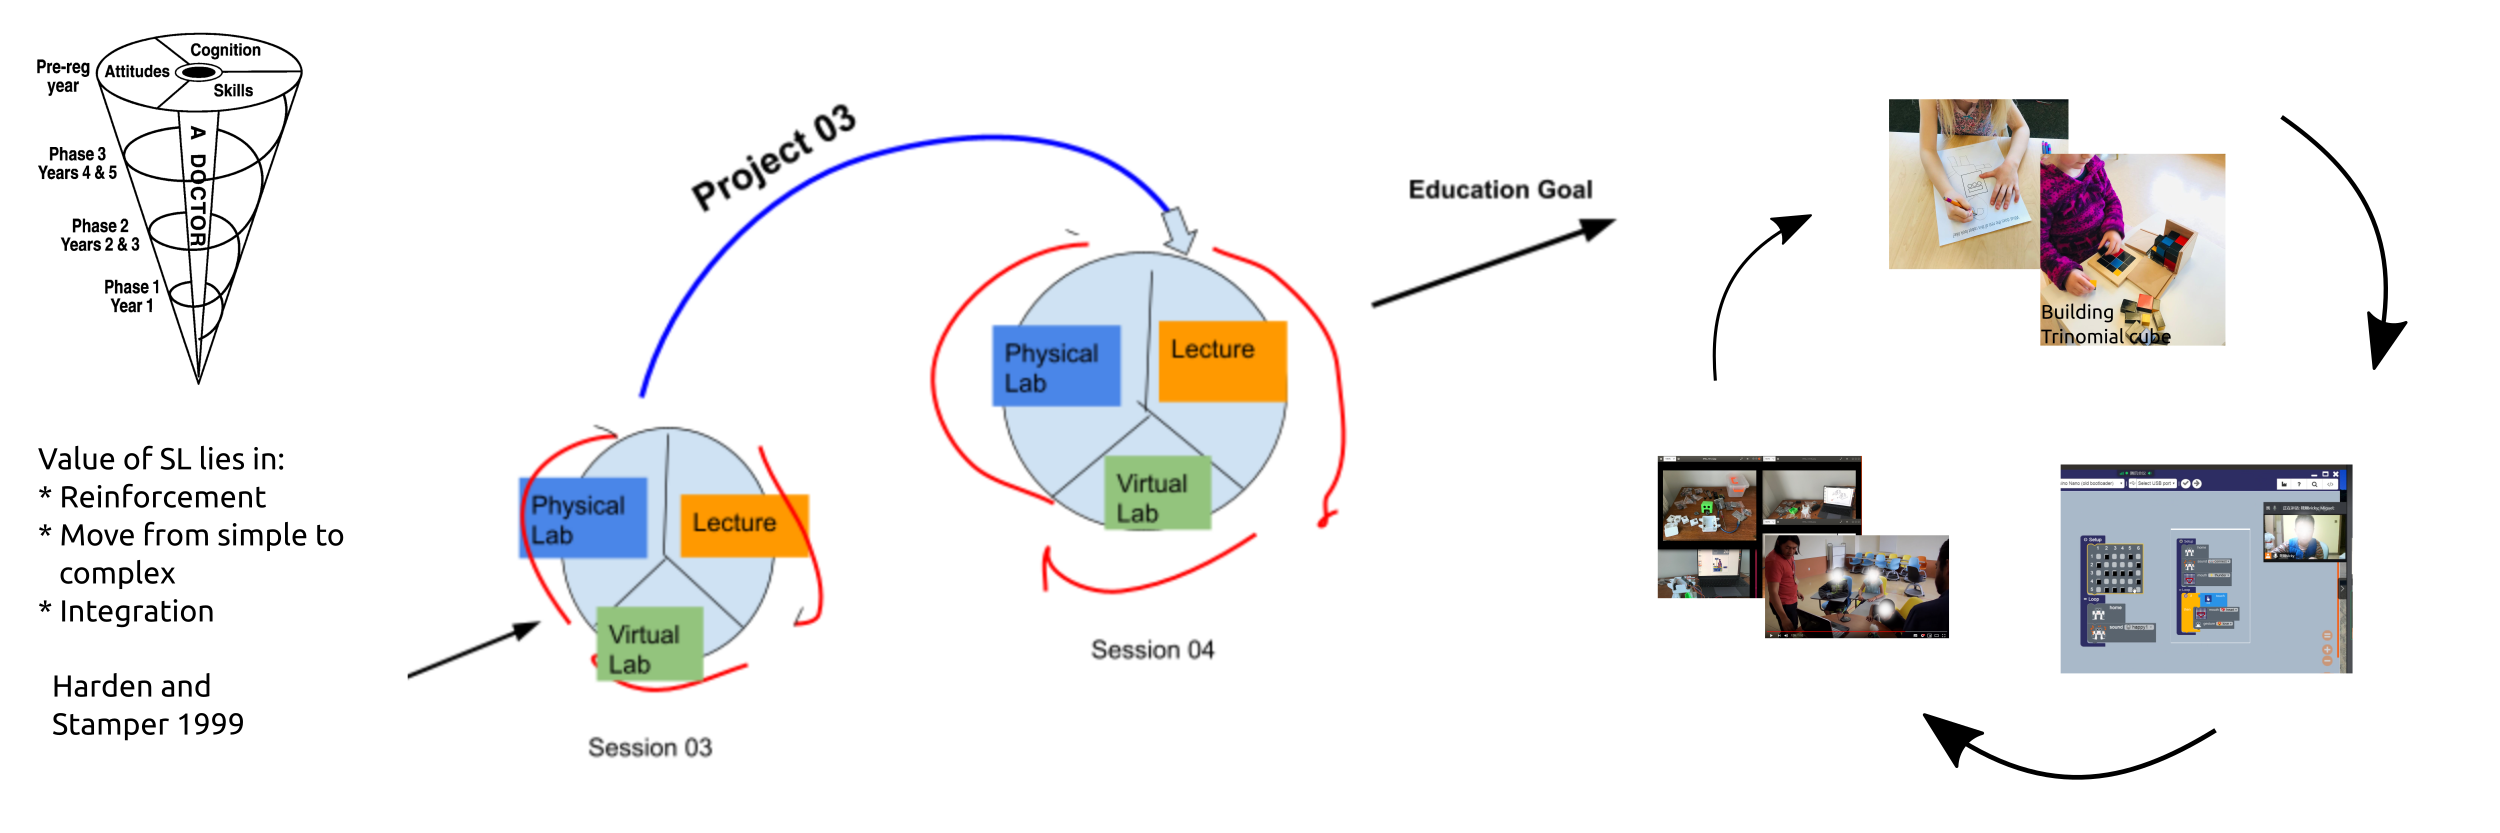
\includegraphics[width=\linewidth]{../figures/curriculum/outputs/drawing-v02.png}  %%GITHUB
    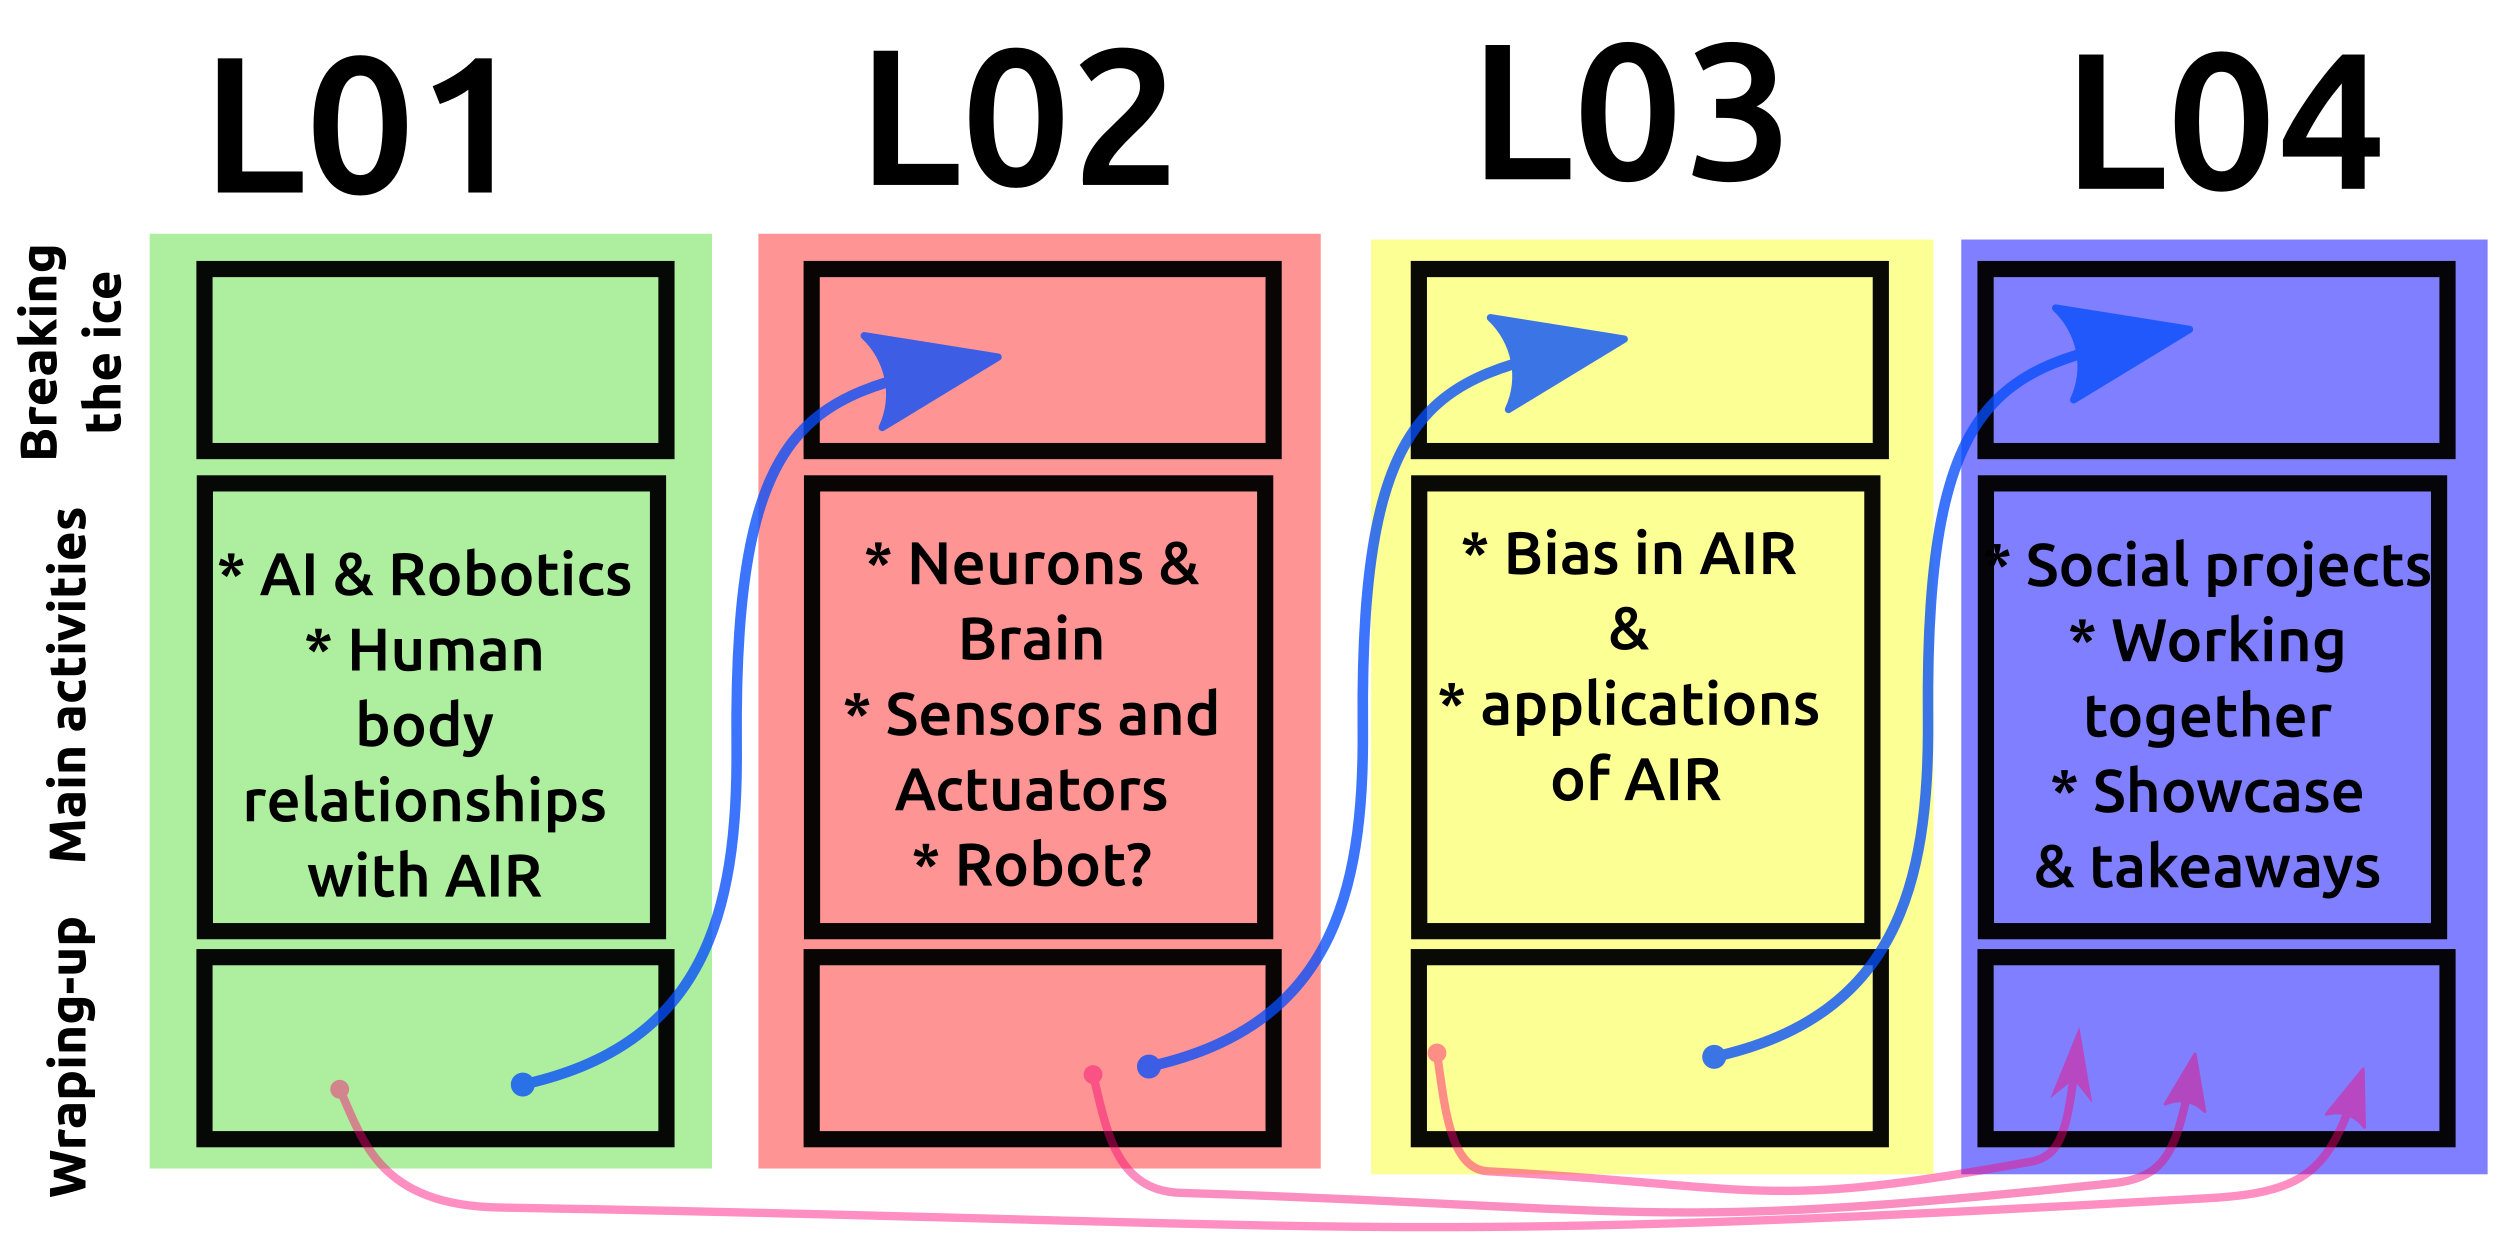
\includegraphics[width=\linewidth]{fig-curriculum.png}  %%OVERLEAF and ARXIV
    \caption{
    Curriculum design with four lessons of 1 hour and a half (L01, L02, L03 and L04).
    The arrows illustrate the connection between the the last and the first part of each lesson as way to summarise the progress of each lesson (blue arrows) and connections with their full curriculum (red arrows).
    }
    \label{fig:curriculum}
\end{figure}
\section{Pilot study: study design and curriculum design}
%%%%%%%%%%%%%%%%%%%%%%%%%%%%%%%%%%%%%%%%%%%%%
% Brieft introduction to this section [MX/TB]
\subsection{Participants}
In this pilot study, we invited 14 participants between the age of 6 to 9 years old. 
During the pilot workshop, only 10 participants 6 male and 4 female of (age in years: mean=8 and std=$\pm$1.61) were able to join the workshops as remained ones were unable to attend due to personal circumstances. 
We also invited four instructors with various experiences levels in teaching subjects to young audiences (two between 5 to 10 years and two with less than 2 years) and one person to lead the logistics of the event.

\subsection{Lessons}
Aiming to create inclusive teaching practices for students, we considered a study design based on procedures, instruments,  data collection and analysis~\cite{du2022}.
Considering the limited human and material resources, we decided to teach four lessons instead of the original ten lessons for the pilot study of this curriculum.

%%%%%%%%%%%%%%%%%%%%%%%%%%%%%%%%%%%%%%%%%%%%%
%% TON~O and DONATO will draft details of the lessons in four paragraphs (or one large paragraph) 
Figure~\ref{fig:curriculum} illustrates the curriculum design for the pilot experiment. 
During the first lesson, we introduced basics concept of human senses and how AI relates to identifying cats and dogs. We were able to use more dynamic activities with protoboards and simple electric circuits so that children can easily learn fundamentals on how a robot works (Figure~\ref{fig:main}d). 
For the second lesson, we presented examples on how AI learn to recognize animals or humans with a tangram activity and gave them a mini introduction to the code that they will use for the robot.
In the third lesson, we adopted a bingo game with key terms from the previous lessons (Figure~\ref{fig:main}b). We 
introduced what is algorithm with an activity of cooking quesadillas where students learnt that everyone can have a different answer given the same instruction.
We also organised activities on action/reaction with different sensors, how sensors work, how to program sensors and examples with the protoboards and circuits.
During the fourth lesson, we closed the course, starting with an activity in the garden where students program their teammates and practice to give instructions to a robot in order to get the wanted result. Then we show them some real life applications of AI and robotics and we grouped participants in three teams so they could program their robots and design their logo (Figure~\ref{fig:main}e). 

\subsection{Surveys}
Considering "Engineering Attitudes Survey" \cite{cunningham2010impact}, we surveyed all participants with same survey, one for the first lesson and one for the last day of the lessons. 
Considering the reduction of time, fatigue and financial compensation, we consider a three-scale Likert chart \cite{jebb2021}, where each statement in our survey has three numbers where 1 is totally disagree; 2: not sure, and 3 totally agree .
See original statements in Table~\ref{tab:questions} and Spanish translation of the statements in Fig~\ref{fig:survey}.

To analyse the results of the survey, we consider the percentages of the responses of each statement from the first and the last lesson and illustrate the results using percentage response of Likert scale charts.
Considering the small sample of participants and the no assumptions to data distributions, we choose the nonparametric Wilcoxon signed-rank test for statistical analysis for answers of pretest and posttest survey \cite{scipy2001}.

% https://www.statstutor.ac.uk/resources/uploaded/mannwhitney.pdf
% The Mann-Whitney U test is a non-parametric test that can be used in place of an
% unpaired t-test. It is used to test the null hypothesis that two samples come from the
% same population (i.e. have the same median) or, alternatively, whether observations in one
% sample tend to be larger than observations in the other. Although it is a non-parametric
% test it does assume that the two distributions are similar in shape.
% Although it is a non-parametric test it does assume that the two distributions are similar in shape.

%%%%%%%%%%%%%%%%%%%%%%%%%%%%%%%%%%%%%%%%%%%%%%%%%%%%%%%%%%%%%%%%%%%%%%
%% TON~O and DONATO will draft statistical analysis of the surveys. added Sat 25 Feb 22:00:33 GMT 2023
% Have a look to this google search for few ideas:
% *  https://www.google.com/search?q=likert+statisc+python&tbm=isch&ved=2ahUKEwiO0KvLz7H9AhURtUwKHZfxDeoQ2-cCegQIABAA&oq=likert+statisc+python&gs_lcp=CgNpbWcQA1DiJFiKMmDfM2gAcAB4AIABUYgBnQSSAQE5mAEAoAEBqgELZ3dzLXdpei1pbWfAAQE&sclient=img&ei=SH76Y46ME5HqsgKX47fQDg&bih=904&biw=1500#imgrc=FDvAEwilQ4OeDM
% * https://www.google.com/search?q=how+to+evaluate+actitudes+statistics+in+surveys+dislake+1+to+5&tbm=isch&ved=2ahUKEwj006q8zrH9AhXSlicCHeBwDdYQ2-cCegQIABAA&oq=how+to+evaluate+actitudes+statistics+in+surveys+dislake+1+to+5&gs_lcp=CgNpbWcQA1DgA1jNEWCZHGgAcAB4AIABQogB_wSSAQIxMZgBAKABAaoBC2d3cy13aXotaW1nwAEB&sclient=img&ei=HH36Y_TVGNKtnsEP4OG1sA0&bih=904&biw=1500

% %%Many thanks TON~O and DONATO, the following is defintely relevant to our work 
% %%We will defintely used it for our large study!
% %%I have added few of your comments to future work 
% A proposal for the statistical analysis of the surveys is as follows.
% \begin{enumerate}
%     \item Select our sample, that is, the people who will answer our surveys. 
%     %(OUR SAMPLE WILL BE ALL THE CHILDREN INVITED TO THE ARTIFICIAL INTELLIGENCE COURSE) 
%     In order to make a representative sample that shows the majority of our student's opinions, it is necessary to define three important points:
%     \begin{itemize}
%         \item Size of our population. 
%         %14 children
%         \item Margin of error (percentage that defines how much the results are close to the opinion of the whole group we are studying).
%         %14.28\% obtenida del numero de estudiantes que teníamos y cuántos lograron hacer los cuestionarios
%         \item Our confidence level (the percentage you think you will be right about which answer our population will select).
%          %90\% that most of the children's answers will change after the class. 
%     \end{itemize}
%     \item Calculate the surveys needed to obtain representative responses from the students with Eq.~\ref{eq:survey}.
%     \begin{equation}
%     \label{eq:survey}
%        n = \frac{N}{[0.05^2 x (N-1)+1]}
%     \end{equation}
%     where, $n=$ number of samples, $N=$ population size and $x=$ number of surveys needed.
%     \item Verify how many surveys were fully completed.
%     \item Given the number of surveys needed and the actual surveys completely made, conclude if the data is reliable and representative.
% \end{enumerate}

\section{Results}
% \subsection{Pilot study}
Four lessons of the designed curriculum were organised on Mondays and Wednesdays in a Mexican town during two weeks of November 2022. 
Instructors helped children in the pilot workshop by creating groups of three to four children.
In the final lesson groups presented their project with their own robot and children with the help of the instructor explained the application of the robot (Figure~\ref{fig:main}).

We only considered 9 participants for the survey as 5 participants were neither in one of the days of the surveys or there were not able to be in person in such days. 
Figure~\ref{fig:results} illustrates percentages or responses of 20 statements from 9 participants for 1 which is totally disagree; 2: not sure, and 3 totally agree.
It can be noted that "S3: I would like a job where I could invent things.", "S11: I would like a job that lets me figure it out how things work"
and ", and "S18: Engineers help make people’s lives better." showed an increase of agreement. 
Whereas "S6: I would like to build and test machines that could help people to walk." and  "S8: I would enjoy a job helping to protect the environment." created less disagreement.
"S17: Scientist help make people’s lives better." resulted in the highest average value whereas "S16: Engineers cause problems in the world." is the lowest average value.
"S19: I think I know what scientists do for their jobs." and "S20: I think I know what engineers do for their jobs." showed both an increase on agreement between participants and decrease in disagreement.

A Wilcoxon T test was used to analyze the results of the survey before and after the survey to see if the engineering attitudes had a significant effect on pre and post survey of the workshop.
The average survey before the test was lower ($\mu$ = 2.194500 $\pm \sigma$ 0.558367 ) compared to the posttest results ($\mu$ = 2.239500 $\pm \sigma$= 0.396796).
There was no statistically significant in the increase of attitudes towards engineering (t=53.5, p= 0.45).
See Appendix section for reproducible Jupyter notebooks of statistical analysis and plots.

% S11: I would like a job that lets me figure it out how things work. 
% S13: I like knowing how things work. 
% Wheres 

\begin{figure}[t]
  \centering
    %\includegraphics[width=\linewidth]{../figures/results/outputs/drawing-v03.png}  %%GITHUB
    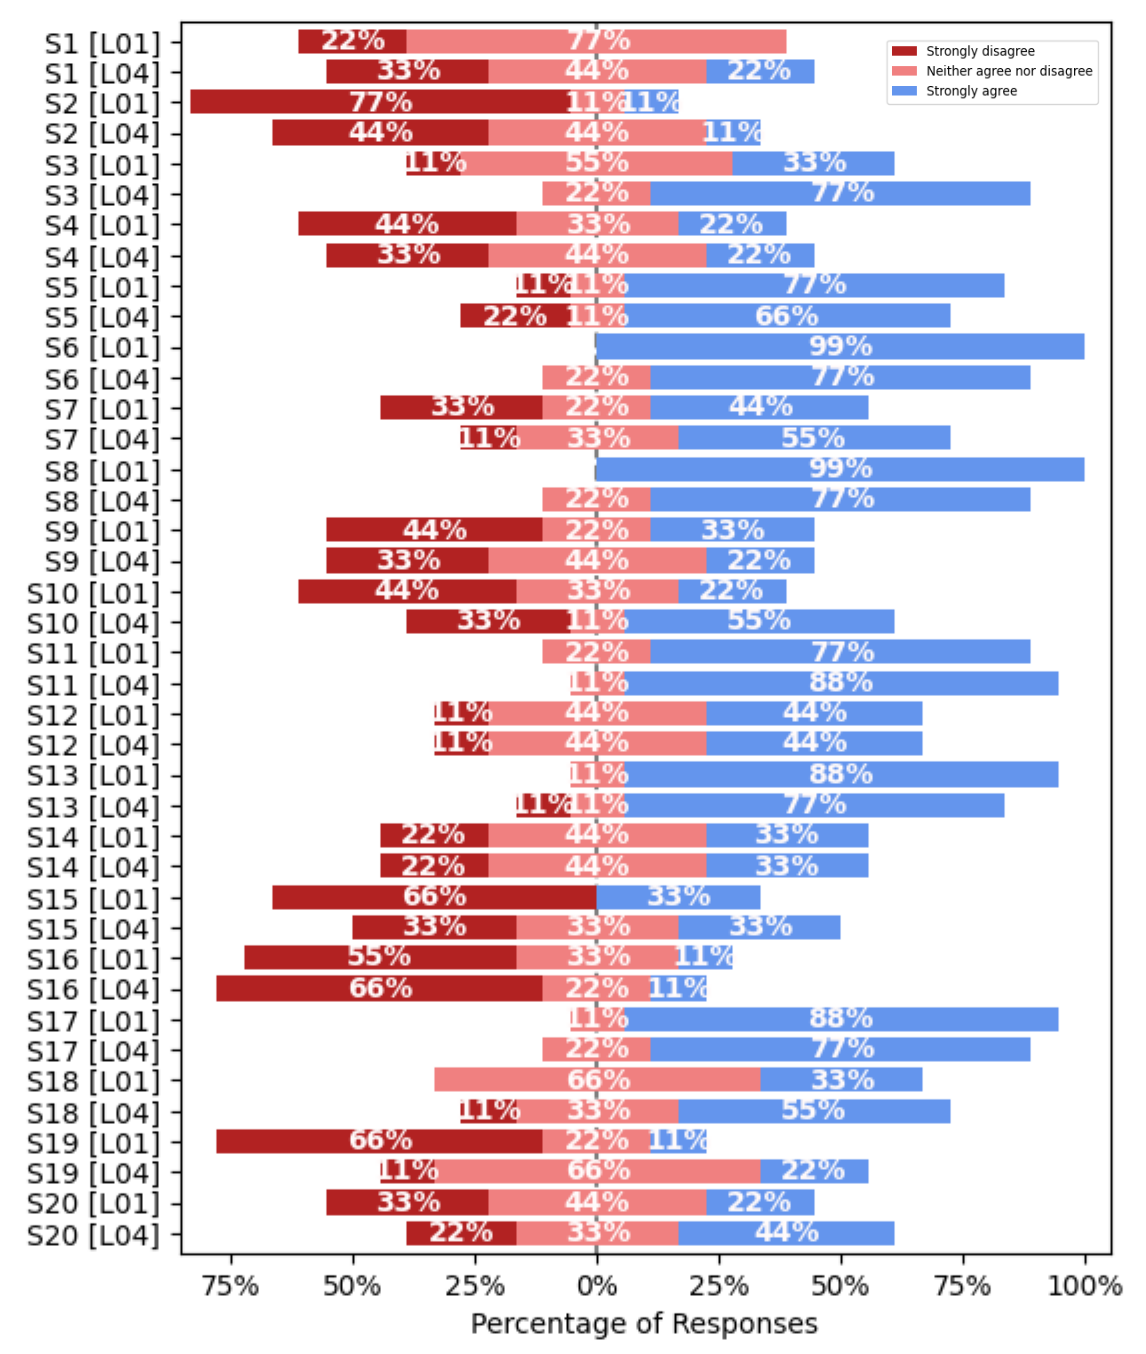
\includegraphics[width=\linewidth]{fig-results.png}  %%OVERLEAF and ARXIV
    \caption{
    Percentages of responses of 9 participants from the survey with 20 statements (S1 to S20) of the first lesson (L01) and the fourth lesson (L04).
    %"S17: Scientist help make people’s lives better." resulted in the highest average value whereas 
    %"S16: Engineers cause problems in the world." is the lowest average value.
    % "S19: I think I know what scientists do for their jobs." and "S20: I think I know what engineers do for their jobs." shows an increase on agreement. 
    See Appendices for further references on the statements of the survey and reproducible jupyter notebooks.
    }
    \label{fig:results}
\end{figure}
% \subsection{Surveys}
% TODO

\section{Conclusions and future work}
%%%%%%%%%%%%%%%%%%%%%%%%
%%% CONCLUSIONS
%%% Please add any conclusions that you saw during the pilot
In this paper, we investigated the challenges of teaching AI and Robotics to young audiences with a pilot study in a Mexican town.
We designed ten lessons but only were able to pilot four lessons due the limited material and human resources. 
We also surveyed participants using Engineering Attitudes Survey from \cite{cunningham2010impact}, and showed the impact on the increase of general agreement of understanding what engineers and scientist do in their jobs using Likert scale charts.
However, statistical analysis suggested no statistically significant in the increase of attitudes towards
engineering  which we think is related to our small sample. 
Also, during the survey we noted that children were not able to read long sentences and were confused about agreement and disagreement terminology in the Likert scale.

We conclude that children and parents had the willingness to join this pilot study by learning new experiences on collaborative and fun activities
based on Montessori education and with low-cost educational robots. 
We also conclude that to be inclusive we would like to include anyone from a potential generation that might be ruled by AI. 
Hence, thanks to these activities we allowed these children coming from low- to mid-income families to learn and be aware of the potential of AI which is crucial in this technological world.

However, the limited and self-funded budget for this project restricted us to prepare and organise a major number of lessons and reach more participants which hopefully will be addressed in future work. 
We will also improve our pretest-posttest survey design with a reliable and representative data and its statistical analysis.

%%%%%%%%%%%%%%%%%%%%%%%%
%%%FUTURE WORK
%%% please add your initials and paragraphs on what you might consider be a good line of research for future work.
%% MX: How to incorporate other examples of bias in AI/Robotics in the context of the Mexican society?

%% The acknowledgments section is defined using the "acks" environment
%% (and NOT an unnumbered section). This ensures the proper
%% identification of the section in the article metadata, and the
%% consistent spelling of the heading.
\begin{acks}
% To everyone involved in this collaborative work.
To Andrea Aguilar-Galindo, Gustavo Barbosa, Donato Badillo-Perez and Antonio Badillo-Perez for volunteering as instructors in the workshops.
To Martha P\'erez and Donato Badillo for their support in organising the pilot of the workshops in their teaching installations. 
To Rocio Montenegro for her contributions with the design of activities based on Montessori education.
To Alex Barco for his feedback to improve the scientific impact of our collaborative work.
To Mercedes P\'erez Mendonza for her feedback on interactive activities.
To Victor Alonso for his feedback on teaching AI to children. 
To Leticia V\'azquez for her support with the translation of surveys and feedback to improve the workshops.
To El\'ias M\'endez Zapata and Abdel Rodriguez Cuapio from Tlaxcala Polytechnic University for their support with the invitation of students and feedback on the hardware design of the robot.
To Xiaoxue Du from MIT Media Labs for her suggestions on the study design. 
To Angel Mandujano, Elva Corona and others who have supported AIR4children project to keep it moving forward. 
\end{acks}

%%
%% The next two lines define the bibliography style to be used, and
%% the bibliography file.
\bibliographystyle{ACM-Reference-Format}
%\bibliography{../references/references} %%GITHUB
%\bibliography{references} %%OVERLEAF
%\bibliography{../../references/references} %%ARXIV
\documentclass[conference]{IEEEtran}
\IEEEoverridecommandlockouts
% The preceding line is only needed to identify funding in the first footnote. If that is unneeded, please comment it out.
\usepackage{cite}
\usepackage{amsmath,amssymb,amsfonts}
\usepackage{algorithmic}
\usepackage{graphicx}
\usepackage{textcomp}
\usepackage{xcolor}
\def\BibTeX{{\rm B\kern-.05em{\sc i\kern-.025em b}\kern-.08em
    T\kern-.1667em\lower.7ex\hbox{E}\kern-.125emX}}
\begin{document}

\title{Conference Paper Title*\\
{\footnotesize \textsuperscript{*}Note: Sub-titles are not captured in Xplore and
should not be used}
\thanks{Identify applicable funding agency here. If none, delete this.}
}

\author{\IEEEauthorblockN{1\textsuperscript{st} Given Name Surname}
\IEEEauthorblockA{\textit{dept. name of organization (of Aff.)} \\
\textit{name of organization (of Aff.)}\\
City, Country \\
email address or ORCID}
\and
\IEEEauthorblockN{2\textsuperscript{nd} Given Name Surname}
\IEEEauthorblockA{\textit{dept. name of organization (of Aff.)} \\
\textit{name of organization (of Aff.)}\\
City, Country \\
email address or ORCID}
\and
\IEEEauthorblockN{3\textsuperscript{rd} Given Name Surname}
\IEEEauthorblockA{\textit{dept. name of organization (of Aff.)} \\
\textit{name of organization (of Aff.)}\\
City, Country \\
email address or ORCID}
\and
\IEEEauthorblockN{4\textsuperscript{th} Given Name Surname}
\IEEEauthorblockA{\textit{dept. name of organization (of Aff.)} \\
\textit{name of organization (of Aff.)}\\
City, Country \\
email address or ORCID}
\and
\IEEEauthorblockN{5\textsuperscript{th} Given Name Surname}
\IEEEauthorblockA{\textit{dept. name of organization (of Aff.)} \\
\textit{name of organization (of Aff.)}\\
City, Country \\
email address or ORCID}
\and
\IEEEauthorblockN{6\textsuperscript{th} Given Name Surname}
\IEEEauthorblockA{\textit{dept. name of organization (of Aff.)} \\
\textit{name of organization (of Aff.)}\\
City, Country \\
email address or ORCID}
}

\maketitle

\begin{abstract}
This document is a model and instructions for \LaTeX.
This and the IEEEtran.cls file define the components of your paper [title, text, heads, etc.]. *CRITICAL: Do Not Use Symbols, Special Characters, Footnotes, 
or Math in Paper Title or Abstract.
\end{abstract}

\begin{IEEEkeywords}
component, formatting, style, styling, insert
\end{IEEEkeywords}

\section{Introduction}
This document is a model and instructions for \LaTeX.
Please observe the conference page limits. 

\section{Ease of Use}

\subsection{Maintaining the Integrity of the Specifications}

The IEEEtran class file is used to format your paper and style the text. All margins, 
column widths, line spaces, and text fonts are prescribed; please do not 
alter them. You may note peculiarities. For example, the head margin
measures proportionately more than is customary. This measurement 
and others are deliberate, using specifications that anticipate your paper 
as one part of the entire proceedings, and not as an independent document. 
Please do not revise any of the current designations.

\section{Prepare Your Paper Before Styling}
Before you begin to format your paper, first write and save the content as a 
separate text file. Complete all content and organizational editing before 
formatting. Please note sections \ref{AA}--\ref{SCM} below for more information on 
proofreading, spelling and grammar.

Keep your text and graphic files separate until after the text has been 
formatted and styled. Do not number text heads---{\LaTeX} will do that 
for you.

\subsection{Abbreviations and Acronyms}\label{AA}
Define abbreviations and acronyms the first time they are used in the text, 
even after they have been defined in the abstract. Abbreviations such as 
IEEE, SI, MKS, CGS, ac, dc, and rms do not have to be defined. Do not use 
abbreviations in the title or heads unless they are unavoidable.

\subsection{Units}
\begin{itemize}
\item Use either SI (MKS) or CGS as primary units. (SI units are encouraged.) English units may be used as secondary units (in parentheses). An exception would be the use of English units as identifiers in trade, such as ``3.5-inch disk drive''.
\item Avoid combining SI and CGS units, such as current in amperes and magnetic field in oersteds. This often leads to confusion because equations do not balance dimensionally. If you must use mixed units, clearly state the units for each quantity that you use in an equation.
\item Do not mix complete spellings and abbreviations of units: ``Wb/m\textsuperscript{2}'' or ``webers per square meter'', not ``webers/m\textsuperscript{2}''. Spell out units when they appear in text: ``. . . a few henries'', not ``. . . a few H''.
\item Use a zero before decimal points: ``0.25'', not ``.25''. Use ``cm\textsuperscript{3}'', not ``cc''.)
\end{itemize}

\subsection{Equations}
Number equations consecutively. To make your 
equations more compact, you may use the solidus (~/~), the exp function, or 
appropriate exponents. Italicize Roman symbols for quantities and variables, 
but not Greek symbols. Use a long dash rather than a hyphen for a minus 
sign. Punctuate equations with commas or periods when they are part of a 
sentence, as in:
\begin{equation}
a+b=\gamma\label{eq}
\end{equation}

Be sure that the 
symbols in your equation have been defined before or immediately following 
the equation. Use ``\eqref{eq}'', not ``Eq.~\eqref{eq}'' or ``equation \eqref{eq}'', except at 
the beginning of a sentence: ``Equation \eqref{eq} is . . .''

\subsection{\LaTeX-Specific Advice}

Please use ``soft'' (e.g., \verb|\eqref{Eq}|) cross references instead
of ``hard'' references (e.g., \verb|(1)|). That will make it possible
to combine sections, add equations, or change the order of figures or
citations without having to go through the file line by line.

Please don't use the \verb|{eqnarray}| equation environment. Use
\verb|{align}| or \verb|{IEEEeqnarray}| instead. The \verb|{eqnarray}|
environment leaves unsightly spaces around relation symbols.

Please note that the \verb|{subequations}| environment in {\LaTeX}
will increment the main equation counter even when there are no
equation numbers displayed. If you forget that, you might write an
article in which the equation numbers skip from (17) to (20), causing
the copy editors to wonder if you've discovered a new method of
counting.

{\BibTeX} does not work by magic. It doesn't get the bibliographic
data from thin air but from .bib files. If you use {\BibTeX} to produce a
bibliography you must send the .bib files. 

{\LaTeX} can't read your mind. If you assign the same label to a
subsubsection and a table, you might find that Table I has been cross
referenced as Table IV-B3. 

{\LaTeX} does not have precognitive abilities. If you put a
\verb|\label| command before the command that updates the counter it's
supposed to be using, the label will pick up the last counter to be
cross referenced instead. In particular, a \verb|\label| command
should not go before the caption of a figure or a table.

Do not use \verb|\nonumber| inside the \verb|{array}| environment. It
will not stop equation numbers inside \verb|{array}| (there won't be
any anyway) and it might stop a wanted equation number in the
surrounding equation.

\subsection{Some Common Mistakes}\label{SCM}
\begin{itemize}
\item The word ``data'' is plural, not singular.
\item The subscript for the permeability of vacuum $\mu_{0}$, and other common scientific constants, is zero with subscript formatting, not a lowercase letter ``o''.
\item In American English, commas, semicolons, periods, question and exclamation marks are located within quotation marks only when a complete thought or name is cited, such as a title or full quotation. When quotation marks are used, instead of a bold or italic typeface, to highlight a word or phrase, punctuation should appear outside of the quotation marks. A parenthetical phrase or statement at the end of a sentence is punctuated outside of the closing parenthesis (like this). (A parenthetical sentence is punctuated within the parentheses.)
\item A graph within a graph is an ``inset'', not an ``insert''. The word alternatively is preferred to the word ``alternately'' (unless you really mean something that alternates).
\item Do not use the word ``essentially'' to mean ``approximately'' or ``effectively''.
\item In your paper title, if the words ``that uses'' can accurately replace the word ``using'', capitalize the ``u''; if not, keep using lower-cased.
\item Be aware of the different meanings of the homophones ``affect'' and ``effect'', ``complement'' and ``compliment'', ``discreet'' and ``discrete'', ``principal'' and ``principle''.
\item Do not confuse ``imply'' and ``infer''.
\item The prefix ``non'' is not a word; it should be joined to the word it modifies, usually without a hyphen.
\item There is no period after the ``et'' in the Latin abbreviation ``et al.''.
\item The abbreviation ``i.e.'' means ``that is'', and the abbreviation ``e.g.'' means ``for example''.
\end{itemize}
An excellent style manual for science writers is \cite{b7}.

\subsection{Authors and Affiliations}
\textbf{The class file is designed for, but not limited to, six authors.} A 
minimum of one author is required for all conference articles. Author names 
should be listed starting from left to right and then moving down to the 
next line. This is the author sequence that will be used in future citations 
and by indexing services. Names should not be listed in columns nor group by 
affiliation. Please keep your affiliations as succinct as possible (for 
example, do not differentiate among departments of the same organization).

\subsection{Identify the Headings}
Headings, or heads, are organizational devices that guide the reader through 
your paper. There are two types: component heads and text heads.

Component heads identify the different components of your paper and are not 
topically subordinate to each other. Examples include Acknowledgments and 
References and, for these, the correct style to use is ``Heading 5''. Use 
``figure caption'' for your Figure captions, and ``table head'' for your 
table title. Run-in heads, such as ``Abstract'', will require you to apply a 
style (in this case, italic) in addition to the style provided by the drop 
down menu to differentiate the head from the text.

Text heads organize the topics on a relational, hierarchical basis. For 
example, the paper title is the primary text head because all subsequent 
material relates and elaborates on this one topic. If there are two or more 
sub-topics, the next level head (uppercase Roman numerals) should be used 
and, conversely, if there are not at least two sub-topics, then no subheads 
should be introduced.

\subsection{Figures and Tables}
\paragraph{Positioning Figures and Tables} Place figures and tables at the top and 
bottom of columns. Avoid placing them in the middle of columns. Large 
figures and tables may span across both columns. Figure captions should be 
below the figures; table heads should appear above the tables. Insert 
figures and tables after they are cited in the text. Use the abbreviation 
``Fig.~\ref{fig}'', even at the beginning of a sentence.

\begin{table}[htbp]
\caption{Table Type Styles}
\begin{center}
\begin{tabular}{|c|c|c|c|}
\hline
\textbf{Table}&\multicolumn{3}{|c|}{\textbf{Table Column Head}} \\
\cline{2-4} 
\textbf{Head} & \textbf{\textit{Table column subhead}}& \textbf{\textit{Subhead}}& \textbf{\textit{Subhead}} \\
\hline
copy& More table copy$^{\mathrm{a}}$& &  \\
\hline
\multicolumn{4}{l}{$^{\mathrm{a}}$Sample of a Table footnote.}
\end{tabular}
\label{tab1}
\end{center}
\end{table}

\begin{figure}[htbp]
\centerline{
\includegraphics{fig1.png}}
\caption{Example of a figure caption.}
\label{fig}
\end{figure}

Figure Labels: Use 8 point Times New Roman for Figure labels. Use words 
rather than symbols or abbreviations when writing Figure axis labels to 
avoid confusing the reader. As an example, write the quantity 
``Magnetization'', or ``Magnetization, M'', not just ``M''. If including 
units in the label, present them within parentheses. Do not label axes only 
with units. In the example, write ``Magnetization (A/m)'' or ``Magnetization 
\{A[m(1)]\}'', not just ``A/m''. Do not label axes with a ratio of 
quantities and units. For example, write ``Temperature (K)'', not 
``Temperature/K''.

\section*{Acknowledgment}

The preferred spelling of the word ``acknowledgment'' in America is without 
an ``e'' after the ``g''. Avoid the stilted expression ``one of us (R. B. 
G.) thanks $\ldots$''. Instead, try ``R. B. G. thanks$\ldots$''. Put sponsor 
acknowledgments in the unnumbered footnote on the first page.

\section*{References}

Please number citations consecutively within brackets \cite{b1}. The 
sentence punctuation follows the bracket \cite{b2}. Refer simply to the reference 
number, as in \cite{b3}---do not use ``Ref. \cite{b3}'' or ``reference \cite{b3}'' except at 
the beginning of a sentence: ``Reference \cite{b3} was the first $\ldots$''

Number footnotes separately in superscripts. Place the actual footnote at 
the bottom of the column in which it was cited. Do not put footnotes in the 
abstract or reference list. Use letters for table footnotes.

Unless there are six authors or more give all authors' names; do not use 
``et al.''. Papers that have not been published, even if they have been 
submitted for publication, should be cited as ``unpublished'' \cite{b4}. Papers 
that have been accepted for publication should be cited as ``in press'' \cite{b5}. 
Capitalize only the first word in a paper title, except for proper nouns and 
element symbols.

For papers published in translation journals, please give the English 
citation first, followed by the original foreign-language citation \cite{b6}.

\begin{thebibliography}{00}
\bibitem{b1} G. Eason, B. Noble, and I. N. Sneddon, ``On certain integrals of Lipschitz-Hankel type involving products of Bessel functions,'' Phil. Trans. Roy. Soc. London, vol. A247, pp. 529--551, April 1955.
\bibitem{b2} J. Clerk Maxwell, A Treatise on Electricity and Magnetism, 3rd ed., vol. 2. Oxford: Clarendon, 1892, pp.68--73.
\bibitem{b3} I. S. Jacobs and C. P. Bean, ``Fine particles, thin films and exchange anisotropy,'' in Magnetism, vol. III, G. T. Rado and H. Suhl, Eds. New York: Academic, 1963, pp. 271--350.
\bibitem{b4} K. Elissa, ``Title of paper if known,'' unpublished.
\bibitem{b5} R. Nicole, ``Title of paper with only first word capitalized,'' J. Name Stand. Abbrev., in press.
\bibitem{b6} Y. Yorozu, M. Hirano, K. Oka, and Y. Tagawa, ``Electron spectroscopy studies on magneto-optical media and plastic substrate interface,'' IEEE Transl. J. Magn. Japan, vol. 2, pp. 740--741, August 1987 [Digests 9th Annual Conf. Magnetics Japan, p. 301, 1982].
\bibitem{b7} M. Young, The Technical Writer's Handbook. Mill Valley, CA: University Science, 1989.
\end{thebibliography}
\vspace{12pt}
\color{red}
IEEE conference templates contain guidance text for composing and formatting conference papers. Please ensure that all template text is removed from your conference paper prior to submission to the conference. Failure to remove the template text from your paper may result in your paper not being published.

\end{document}
 %% uncomment for arxiv version

%%%
%%% If your work has an appendix, this is the place to put it.

\newpage

\section*{Appendices}
\appendix

\section*{Surveys}
Figure~\ref{fig:survey} shows survey layout document and table~\ref{tab:questions} presents 20 statements of the survey.
\begin{figure} %[h]
  \centering
    %\includegraphics[width=\linewidth]{../figures/surveys/outputs/drawing-v00.png}  %%GITHUB
    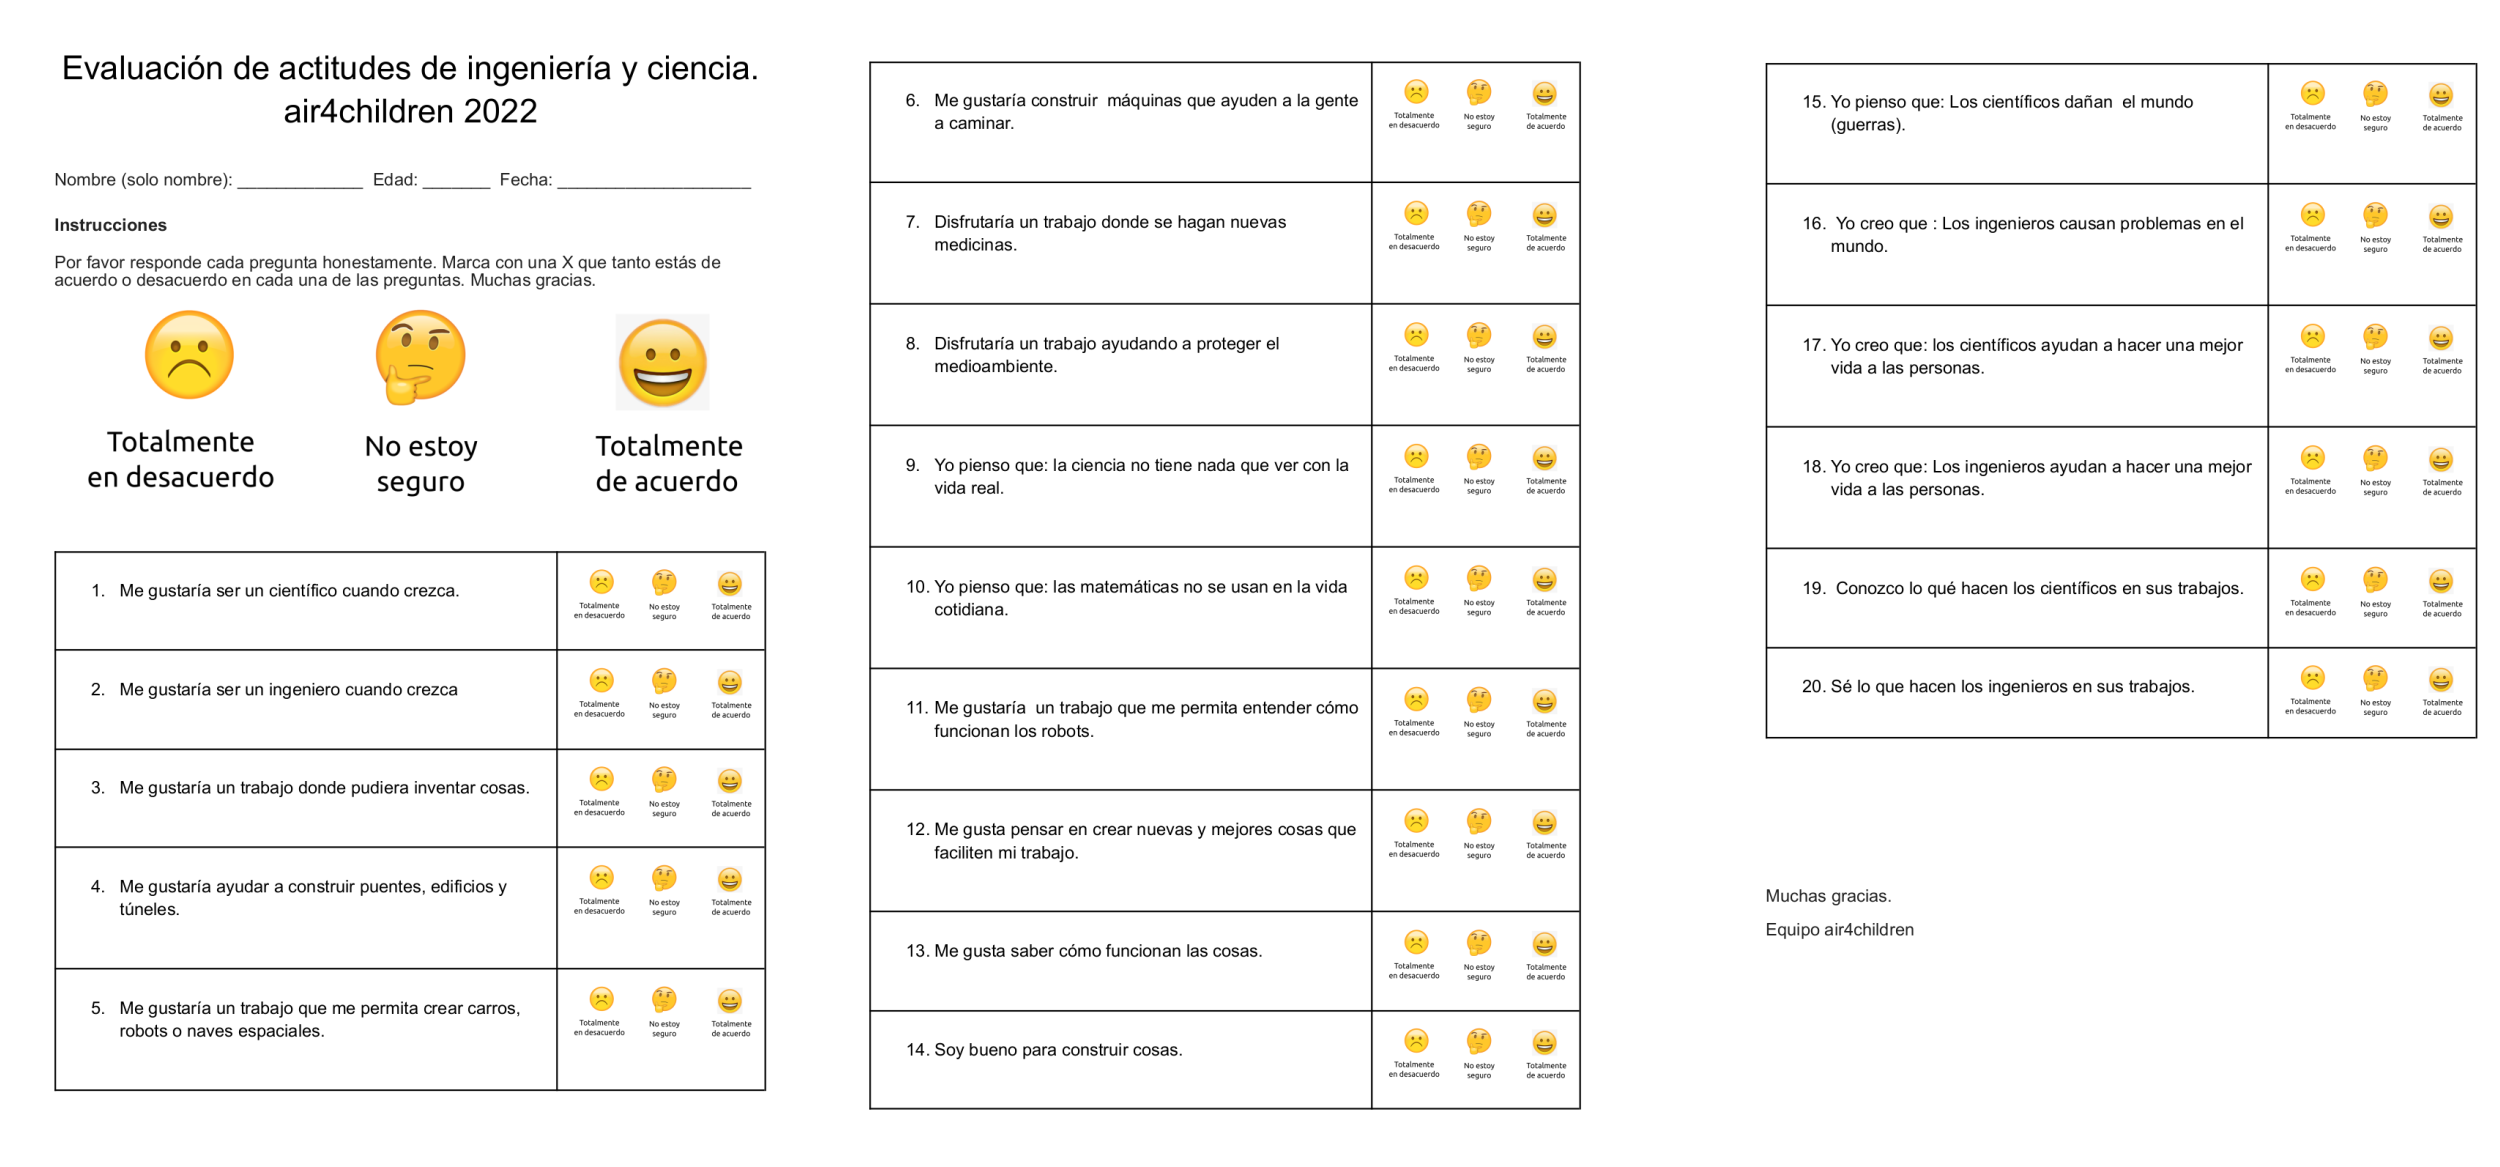
\includegraphics[width=\linewidth]{fig-surveys.png}  %%OVERLEAF and ARXIV 
    \caption{
    Survey in Spanish with 20 statements.
	Statements were translated from English to Spanish from the "Engineering Attitudes Survey" \cite{cunningham2010impact}.
    }
    \label{fig:survey}
\end{figure}

\begin{table*}[h]
  \caption{Statements in the survey from "Engineering Attitudes Survey" \cite{cunningham2010impact}.
}
  \label{tab:questions}
  \begin{tabular}{ll}
    \toprule
    Number & Statements \\
    \midrule
    S1 & I would enjoy being a scientist when I grow up \\
    S2 & I would enjoy being an engineer when I grow up.  \\
    S3 & I would like a job where I could invent things. \\
    S4 & I would like to help to plan bridges, skyscrapers, and tunnels. \\
    S5 & I would like a job that lets me design a cars. \\   
    S6 & I would like to build and test machines that could help people to walk. \\
    S7 & I would enjoy a job helping to make new medicines. \\
    S8 & I would enjoy a job helping to protect the environment. \\
    S9 & Science has nothing to do with real life. \\
    S10 & Math has nothing to do with real life. \\
    S11 & I would like a job that lets me figure it out how things work. \\
    S12 & I like thinking of new and better ways of doing things. \\
    S13 & I like knowing how things work. \\
    S14 & I am good at putting things together. \\
    S15 & Scientist cause problems in the world. \\
    S16 & Engineers cause problems in the world. \\
    S17 & Scientist help make people’s lives better. \\
    S18 & Engineers help make people’s lives better. \\
    S19 & I think I know what scientists do for their jobs. \\
    S20 & I think I know what engineers do for their jobs. \\
    \bottomrule
  \end{tabular}
\end{table*}


\section*{Jupyter notebooks}
Figure~\ref{fig:notebooks} shows Jupyter notebooks which are available at \\ \url{https://github.com/air4children/dei-hri2023/}
\begin{figure}[h]
  \centering
    %\includegraphics[width=\linewidth]{../figures/jupyter-notebooks/outputs/drawing-v00.png}  %%GITHUB
    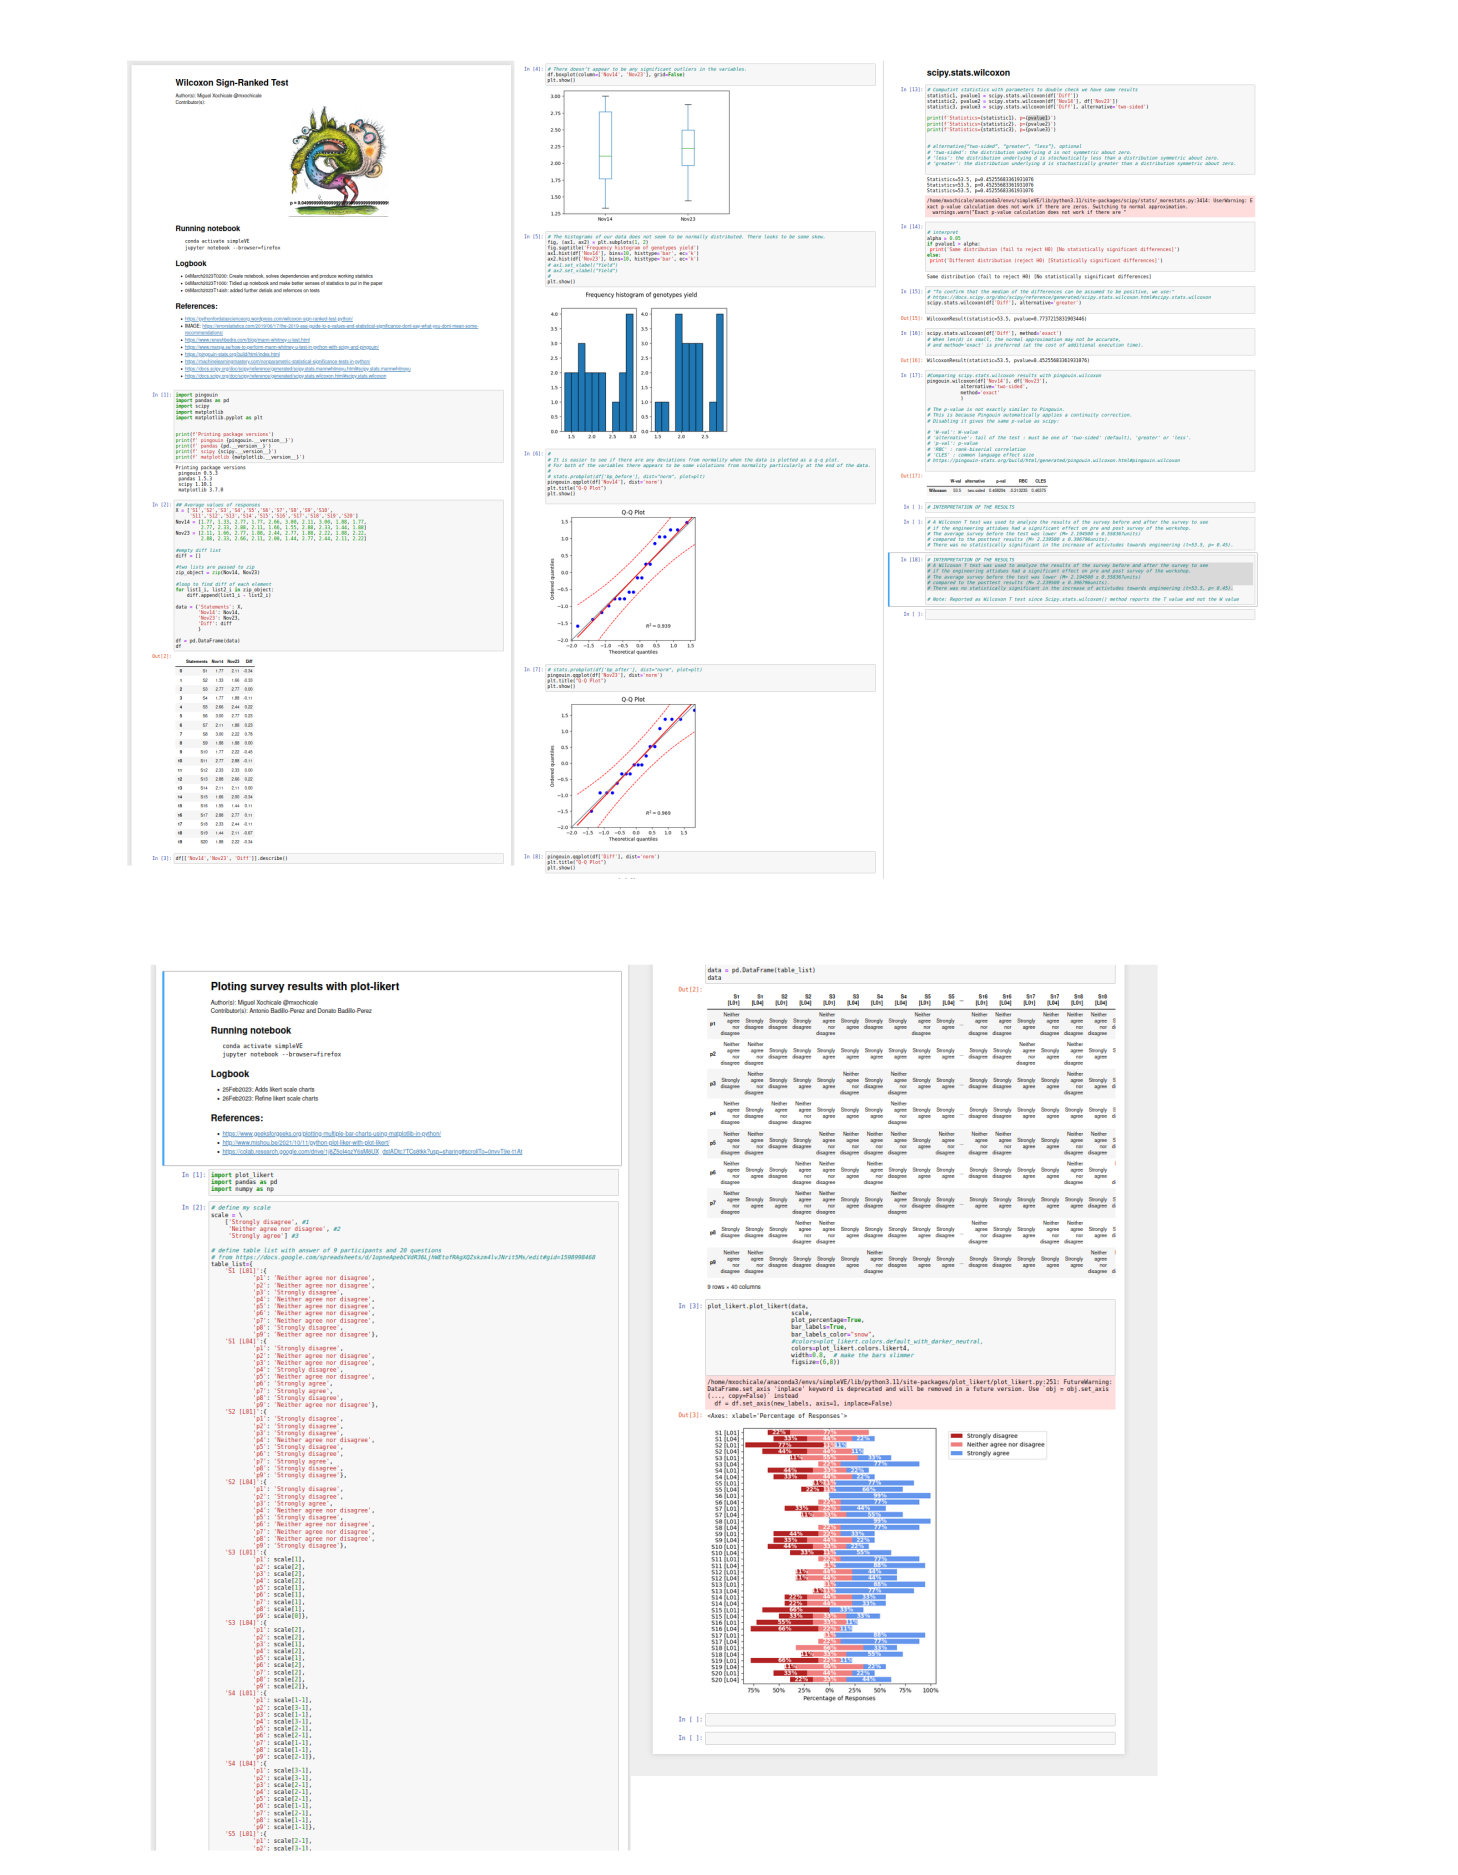
\includegraphics[width=\linewidth]{fig-jupyter-notebooks.png}  %%OVERLEAF and ARXIV 
    \caption{
    Jupyter notebooks are available at \url{https://github.com/air4children/dei-hri2023/}
    }
    \label{fig:notebooks}
\end{figure}

%\subsection{Part One}
%

%\subsection{Part Two}
%
%Etiam commodo feugiat nisl pulvinar pellentesque. Etiam auctor sodales
%ligula, non varius nibh pulvinar semper. Suspendisse nec lectus non
%ipsum convallis congue hendrerit vitae sapien. Donec at laoreet
%eros. Vivamus non purus placerat, scelerisque diam eu, cursus
%ante. Etiam aliquam tortor auctor efficitur mattis.
%


\end{document}
\endinput
%%
